% ----------------------------------------------------------
\chapter{Metodologia}
% ----------------------------------------------------------
	Nesta seção do trabalho, definimos a área geográfica do estudo, assim como os conjuntos de dados levantados para as análises que servirão de base para as simulações de trajetória e dispersão dos poluentes, bem como detalhamentos sobre a obtenção das mesmas.
	
\section{Área de Estudo}
\subsection{Santa Catarina}  
	O estado de Santa Catarina, situado na região sul do Brasil, entre as latitudes de 25º57'41" e 29º23'55", e longitudes 48º19'37" e 53º50'00" possui uma paisagem muito diversificada, com uma faixa litorânea sobre o Oceano Atlântico, o estado também conta com regiões de Serra, Planaltos e Planícies que se estendem até a divisa com a Argentina. Sua mesorregião oeste, conforme indicado na Figura 7 como foco do estudo, situada entre os Planaltos dos rios Uruguai e Iguaçu, possui aproximadamente 23.710 km2 e possui temperaturas médias entre 13 e 16 °C e valor médio de precipitação entre 420 e 480 mm para o período de inverno do hemisfério sul, compreendido entre 21 de junho e 22 de setembro \autocite{santacatarina_seplan2016}.
	
	De acordo com o Atlas Climático proposto por \autocite{oliveira2024}, as mesorregiões Oeste/Extremo Oeste não possuem estações seca e úmida bem definidas, e seus menores acumulados de precipitação se encontram ao longo do inverno, fenômeno atrelado à presença de bloqueios atmosféricos causados por sistemas de alta pressão que impedem a passagem de sistemas frontais. Quanto aos maiores acumulados de precipitação, o autor atribui a influência do SAALJ no transporte de umidade proveniente da Amazônia para a região sul do continente, que contribui com o aumento de eventos convectivos e de Sistemas Convectivos de Mesoescala na região.
	
\begin{figure}[htb]
	\begin{center}
		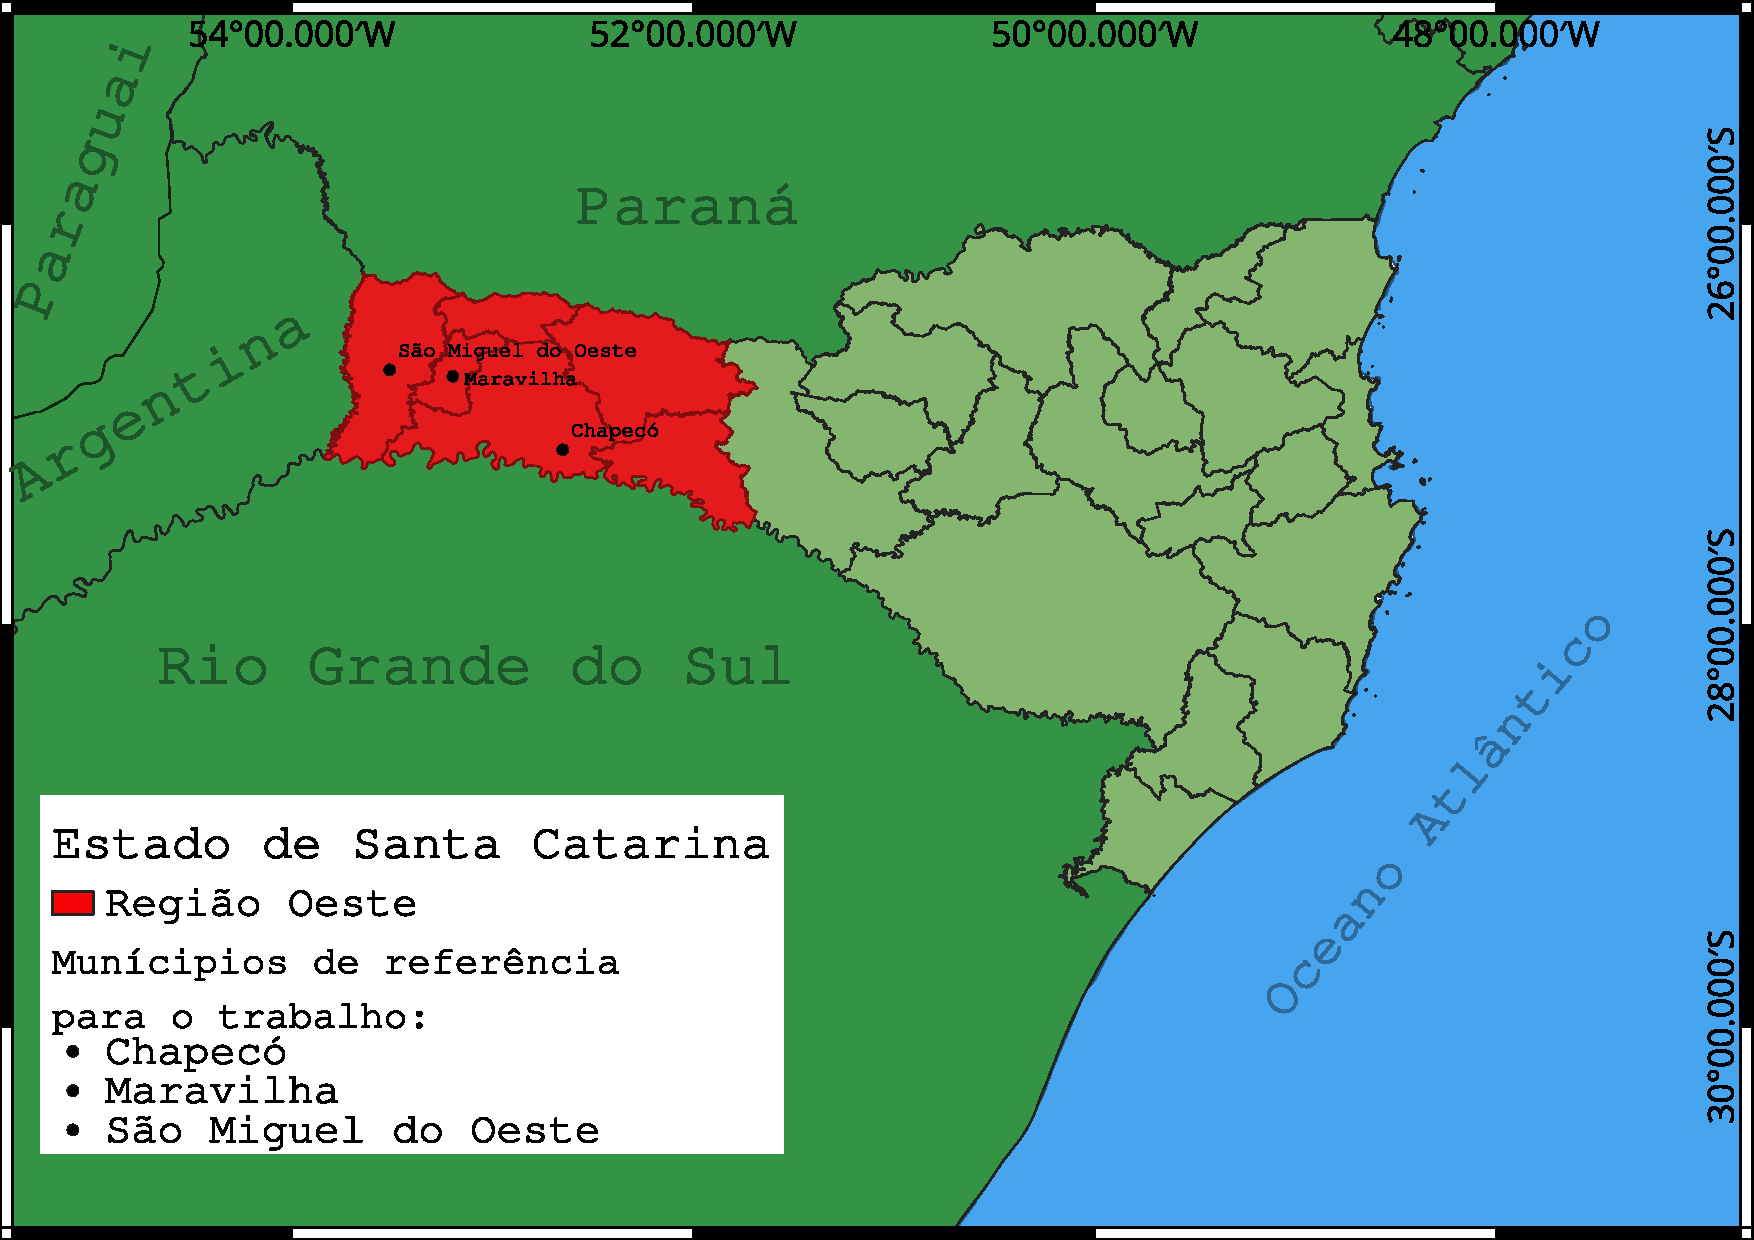
\includegraphics[width=\textwidth]{images/figura7.pdf}
	\end{center}
	\caption{Mapa do estado de Santa Catarina com destaque para a região oeste. Elaboração do autor com dados do IBGE.}
\end{figure}

\section{Dados Utilizados}
\subsection{Reanálise \textit{Copernicus Atmosphere Monitoring Service} (CAMS) EAC4}

	Produto também disponibilizado pelo ECMWF (European Centre for Medium-Range Weather Forecasts), a reanálise CAMS (Copernicus Atmosphere Monitoring Service) é composta por uma assimilação de dados referentes à composição da atmosfera, com foco na identificação de aerossóis e espécies químicas. O conjunto conta com dados em escala de 3 horas, cobrindo toda a superfície terrestre com resolução de 0.75° e duas diferentes formas de espacializar o dado verticalmente (por níveis de pressão e 60 níveis próprios do produto). As variáveis disponíveis possuem alguma semelhança com as da reanálise ERA5 (vento e temperatura, por exemplo) mas se distingue pelo detalhamento nas espécies químicas e quantificações de aerossóis \autocite{inness2019}. Para o presente trabalho, serão analisadas as seguintes variáveis:
	\begin{itemize}
		\item Profundidade Óptica de Black Carbon a 550 nm (Black Carbon AOD) (Adimensional)
		\item Material Particulado com até 1 nm de diâmetro (PM$_{1}$) ($kgm^{3}$)
		
	\end{itemize}

\subsection{Reanálise ERA5}

	Criada e mantida pelo European Centre for Medium-Range Weather Forecasts (ECMWF), a reanálise ERA-5 conta com diversas variáveis meteorológicas agrupadas em uma grade espacial de 31km, distribuídas em 137 níveis distintos de pressão com registros desde o ano de 1940. Para o presente trabalho foram coletados dados entre as datas 11/09/2024 e 13/09/2024, com resolução horária nos seguintes conjuntos de reanálise \autocite{hersbach2020}:
	
	\begin{itemize}
		\item \textit{ERA5 hourly data on pressure levels from 1940 to present}
		\begin{itemize}
			\item Componente zonal do vento ($ms^{-1}$)
			\item Componente meridional do vento ($ms^{-1}$)
			\item Velocidade vertical do vento($Pas^{-1}$)
			\item Umidade relativa (\%)
			\item Geopotencial ($m^{2}s^{-1}$)
			\item Temperatura (K)
		\end{itemize}
		\item \textit{ERA5 hourly data on single levels from 1940 to present}
		\begin{itemize}
			\item Temperatura a 2 metros do solo (K)
			\item Pressão à superfície (Pa)
			\item Precipitação total (m)
			\item Geopotencial ($m^{2}s^{-1}$)
		\end{itemize}
	\end{itemize}
	
\subsection{Satélite Goes-16}
	Operado pela \textit{National Oceanic and Atmospheric Administration} (NOAA) e pela \textit{National Aeronautics and Space Administration} (NASA), o satélite GOES-16 monitora os continentes americanos norte e sul, bem como oceanos que os delimitam através de uma órbita geoestacionária que o posiciona de forma constante com relação à essa face específica do planeta terrestre. Dentre suas diferentes aplicações, o satélite conta com um sensor multiespectral de alta resolução espacial e temporal que consegue captar dados em 16 bandas diferentes do espectro eletromagnético \autocite{goodman2019goes}. 
	
	 
	Em especial, o canal 13 (comumente referenciado como Infravermelho Limpo, centrado em 10,3 $\mu m$) se destaca como ferramenta essencial para análises de condições meteorológicas por permitir a identificação do topo de nuvens independente do ciclo diurno, com isso, torna-se possível a demarcação de sistemas sinóticos \autocite{schmit2017closer}.
	
\subsection{\textit{CAMS Global Fire Assimilation System} (GFAS)}
\label{subsec:cams-gfas}

	Partindo das observações de Potência Radiativa do Fogo obtidas feitas por satélites, a reanálise GFAS disponibiliza informações sobre a localização, intensidade relativa e emissões estimadas de queima de biomassa e incêndios de vegetação. O resultado é uma reanálise com 0.1° de resolução espacial e resolução temporal de um dia \autocite{kaiser2012}. Para o presente trabalho foram utilizadas as seguintes variáveis:
	\begin{itemize}
		\item Altura de Injeção ($m$)
		\item Base da Pluma acima da Superfície ($m$)
		\item Fluxo de queima de Black Carbon ($kgm^{-2}s^{-1}$)
		\item Fluxo de queima de Material Particulado Total ($kgm^{-2}s^{-1}$)
		\item Fluxo de queima de Dióxido de Carbono ($kgm^{-2}s^{-1}$)
	
	\end{itemize}
\subsection{Modelo HYSPLIT}
	O Hybrid Single-Particle Lagrangian Integrated Trajectory  (HYSPLIT) é um modelo lagrangiano de trajetórias criado pelo Air Source Laboratory, administrado pela National Oceanic and Atmospheric Administration (NOAA) dos Estados Unidos, com o qual é possível calcular transporte e dispersão atmosféricos. Suas aplicações variam entre o rastreio e previsão da liberação de material radioativo, poeira transportada pelo vento e fumaça liberada por queimadas. Apesar do nome, o modelo acaba por misturar as abordagens lagrangeanas e eulerianas no seu método de cálculo: a primeira é utilizada na descrição da trajetória das partículas/massas de ar ao longo da simulação, enquanto o referencial euleriano é empregado para calcular as concentrações do poluente em uma grade fixa.
	
	O fluxo de uso do modelo consiste no pré-processamento de dados meteorológicos que servirão de base para a execução das simulações, sendo possível simular trajetórias tanto avançando quanto retrocedendo no tempo (comumente referidas como forward e backward trajectories, respectivamente). Também é possível executar simulações de transporte, dispersão e deposição de poluentes atmosféricos alimentando o modelo com informações sobre as propriedades físico-químicas e taxas de emissão do aerossol em questão \autocite{stein2015}.
	
\subsection{Procedimentos}
	\subsubsection{Delimitação Espacial e Temporal}
	Como primeiro passo de execução do trabalho, foram avaliados dados da reanálise ERA5 em conjunto com imagens do satélite GOES-16 afim de estabelecer o padrão sinótico do evento. Em seguida, a reanálise CAMS foi averiguada com foco nas variáveis de profundidade óptica (AOD), buscando os períodos e pontos de máxima ao longo do estado de Santa Catarina para definir as coordenadas e datas de simulação no modelo HYSPLIT.
	
	\subsubsection{Análise Sinótica}
	Com o objetivo de identificar os padrões meteorológicos que contribuíram para a intensidade do fenômeno de transporte dos aerossóis, bem como sua duração anômala sobre o estado de Santa Catarina, foram utilizados dados do modelo ERA-5 em conjunto com imagens do satélite Goes-16 no canal 13 em intervalos de seis horas, afim de estabelecer o padrão sinótico da época. 

	\subsubsection{Trajetórias}
	
	Após produzir os mapas de profundidades ópticas, a reanálise ERA 5 foi utilizada como fonte dos dados meteorólogicos no modelo HYSPLIT. Primeiro, para as simulações de trajetória, foi necessário agrupar os dados de superfície com os dados de níveis de pressão através da ferramenta CDO \autocite{INPE2016mtc}. Em seguida, o arquivo no formato \textit{grib} foi convertido para o formato \textit{ARL}, nativo do modelo HYSPLIT.
	
	Utilizando os resultados provenientes das análises do modelo CAMS e os registros midiáticos fornecidos por \textcite{epagri2024chuvapreta}, foram definidos três municípios como pontos de referência para as trajetórias reversas das parcelas de ar: Chapecó, Maravilha e São Miguel do Oeste. Como o intuito é analisar o movimento das parcelas em função do SAALJ, foram utilizados scripts computacionais na linguagem \textit{Python} para estimar as alturas acima do nível do solo equivalentes aos níveis de pressão de 750, 800 e 850 hPa para cada um dos pontos. Para tal, os dados de geopotencial obtidos na reanálise foram convertidos para metros acima do nível do solo ($m agl$) da seguinte maneira, de acordo com \textcite{holton2012introduction}:
	\begin{equation}
		Z_{m agl} = \frac{\Phi(p)}{g} - z_{elevação}.
	\end{equation}
	
	Onde $g = 9{,}80665 \text{ms}^{2}$, $\Phi(p)$ é a altura geopotencial da camada de pressão desejada e $z_{elevação}$ é a altura média dos municípios acima do nível do mar. Os respectivos valores inseridos na rodada do modelo se encontram dispostos na Tabela \ref{table:Tabela 1}. A data selecionada para o fim da trajetória foi 13 de setembro de 2024 e a simulação teve duração total de -72h.
	

	
	\begin{table}
		\begin{center}
			\begin{tabular}{ ccc } 
				\hline
				Município & Lat Lon (°) & Níveis de altura (m-agl) \\
				\hline
				\multirow{3}{4em}{Chapecó} &  & 1850.04 \\ 
				& -27.0   -52.7 & 1305.15 \\ 
				&  & 786.94 \\ 
				\hline
								\multirow{3}{4em}{Maravilha} &  & 1976.17 \\ 
				& -26.77   -52.21 & 1432.56 \\ 
				&  & 915.06 \\ 
				\hline
								\multirow{3}{4em}{São Miguel do Oeste} &  & 1850.04 \\ 
				& -26.72   -53.51 & 1305.15 \\ 
				&  & 786.94 \\ 
				\hline
			\end{tabular}
		\end{center}
		\caption{Dados de entrada para as rodadas de trajetória reversa no modelo HYSPLIT.}
		\label{table:Tabela 1}
	\end{table}
	
	\subsubsection{Dispersão}
	Para a simulação de dispersão, foi necessário definir pontos de emissão de aerossóis provenientes de queimadas, que foram obtidos através da reanálise GFAS. Foi aplicada uma conversão nas variáveis de fluxo de emissão dos poluentes ($kgm^{-2}s^{-1}$), com o intuito de obter um valor para a taxa de emissão ($kgs^{-1}$) através da seguinte equação:
	
	\begin{equation}
		E = F * A
	\end{equation}
	
	Para a obtenção da área necessária para o cálculo, foi empregado um algoritmo computacional na linguagem \textit{Python} onde o gradeamento da reanálise é convertido da unidade de graus para $m^{2}$. Após essa conversão, foram selecionados os cinco maiores pontos de emissão de cada dia dentro da área horizontal de ocorrência do JBN definida a partir dos dados do ERA5. Neste caso, a dispersão será no sentido \textit{forward}, para que seja possível analisar quais plumas foram melhor transportadas para as regiões de interesse, além da concentração das mesmas.
	
	Para cada um dos dias compreendidos dentro da simulação, foram selecionados os cinco maiores pontos de emissão com altura de injeção da pluma mais próxima do nível de 800 hPa. Os dados de emissão implementados no modelo estão descritos na Tabela \ref{table:dados_focos}.
	
	
	\begin{table}[htbp]
		\centering
		\vspace{8pt}
		\small
		\begin{tabular}{ccccccrcc}
			\toprule
			\textbf{Data} & \textbf{Lat ($^\circ$)} & \textbf{Lon ($^\circ$)} & \textbf{Alt} (\unit{\meter}) & \textbf{Taxa} (\unit{\per\hour}) & \textbf{Área} (\unit{\meter\squared}) & \textbf{Calor} (\unit{\watt}) \\
			\midrule
			  & -18.550 & -57.750 & 1425.6 & 32\,250.50 & 117\,219\,411.3 & 2\,326\,214\,656.0 \\
			\multirow{3}{*}{2024-09-09} & -22.750 & -53.650 & 1896.3 & 31\,279.33 & 114\,023\,802.7 & 1\,381\,107\,840.0 \\
			  & -11.050 & -54.950 & 1433.3 & 25\,135.51 & 121\,350\,810.5 & 803\,256\,448.0 \\
			 & -9.350  & -55.050 & 1747.9 & 25\,031.70 & 122\,000\,433.6 & 799\,939\,136.0 \\
			 & -18.550 & -57.650 & 1564.9 & 19\,741.50 & 117\,219\,411.3 & 1\,423\,945\,856.0 \\
			\midrule
			 & -22.750 & -53.650 & 1577.3 & 23\,411.63 & 114\,023\,802.7 & 1\,033\,717\,568.0 \\
			\multirow{3}{*}{2024-09-10} & -22.750 & -53.550 & 1598.6 & 18\,932.48 & 114\,023\,802.7 & 605\,025\,920.0 \\
			 & -11.050 & -54.950 & 1433.3 & 14\,379.62 & 121\,350\,810.5 & 459\,530\,176.0 \\
			 & -15.850 & -63.850 & 1942.9 & 12\,999.00 & 118\,942\,208.0 & 415\,409\,600.0 \\
			 & -15.550 & -55.550 & 1193.9 & 9\,496.09  & 119\,117\,392.9 & 684\,949\,184.0 \\
			\midrule
			 & -10.850 & -53.050 & 1969.4 & 53\,027.97 & 121\,432\,793.1 & 1\,694\,617\,216.0 \\
			\multirow{3}{*}{2024-09-11} & -15.050 & -60.350 & 1109.1 & 25\,441.96 & 119\,402\,108.3 & 1\,835\,117\,568.0 \\
			 & -15.950 & -57.650 & 1866.7 & 18\,326.35 & 118\,883\,088.2 & 1\,321\,871\,872.0 \\
			 & -15.550 & -62.550 & 1781.5 & 12\,427.81 & 119\,117\,392.9 & 397\,156\,128.0 \\
			 & -15.950 & -57.550 & 1948.4 & 9\,241.93  & 118\,883\,088.2 & 666\,616\,128.0 \\
			\midrule
			 & -15.950 & -57.650 & 1769.9 & 22\,138.54 & 118\,883\,088.2 & 1\,596\,843\,264.0 \\
			\multirow{3}{*}{2024-09-12} & -14.750 & -65.250 & 1700.0 & 17\,709.22 & 119\,568\,574.3 & 565\,934\,272.0 \\
			 & -10.850 & -53.050 & 1969.4 & 14\,855.68 & 121\,432\,793.1 & 474\,743\,424.0 \\
			 & -11.950 & -52.950 & 1281.8 & 12\,537.89 & 120\,963\,605.8 & 400\,673\,920.0 \\
			 & -19.550 & -58.750 & 1850.0 & 10\,840.64 & 116\,515\,070.5 & 781\,930\,688.0 \\
			\bottomrule
		\end{tabular}
		\caption{Registros diários de focos, localização e taxa de emissão de calor.}
		\label{table:dados_focos}
	\end{table}
	
	Além dos dados meteorológicos e de emissões, foi necessário implementar propriedades físico-químicas para cada uma das categorias de aerossol analisadas no trabalho. Mediante a disponibilidade dos dados de emissão do GFAS, o presente trabalho gerou simulações para aerossóis do tipo \textit{Black Carbon} e $PM_{2.5}$, cujas parametrizações estão dispostas na Tabela \ref{table:fsc_qmc}.
	
	\begin{table}[htbp]
		\centering
		\begin{tabular}{llccc}
			\toprule
			\textbf{Parâmetro no \texttt{CONTROL}}  & \textbf{Valor ($\text{PM}_{2.5}$)} & \textbf{Valor (BC)} & \textbf{Unidade} \\
			\midrule
			Identificador do Poluente  & \texttt{PM25} & \texttt{BC} & -- \\
			Diâmetro da Partícula  ($d_p$) & 0.5 & 0.15 & $\mu\text{m}$ \\
			Densidade da Partícula  ($\rho$) & 1.5 & 1.0 & $\text{g/cm}^3$ \\
			Fator de Forma  ($\gamma$) & 1.0 & 1.0 & -- \\
			Velocidade de Deposição Seca  ($V_d$) & 0.0 & 0.0 & $\text{m/s}$ \\
			Constante de Henry  ($H$) & $1.0 \times 10^{4}$ & $1.0 \times 10^{-5}$ & $\text{M/atm}$ \\
			Razão de Varredura \emph{In-Cloud}  ($S$) & $3.2 \times 10^{5}$ & $8.0 \times 10^{-5}$ & $\text{L/L}$ \\
			Constante \emph{Below-Cloud}  & $1.0 \times 10^{-5}$ & $8.0 \times 10^{-5}$ & $\text{s}^{-1}$ \\
			Decaimento Químico  & 0.0 & 0.0 & dias \\
			Resuspensão  & 0.0 & 0.0 & $\text{m}^{-1}$ \\
			\bottomrule
		\end{tabular}
		\caption{Comparação dos parâmetros físicos e de deposição configurados no arquivo CONTROL do HYSPLIT para $\text{PM}_{2.5}$ e Black Carbon (BC).}
		\label{table:fsc_qmc}
	\end{table}
	
	Após definidas as propriedades físico-químicas, os parâmetros de grade definidos para as rodadas de dispersão estão apresentados na Tabela \ref{table:grid_hysplit}.
	
	\begin{table}[htbp]
		\centering

		\begin{tabular}{llcc}
			\toprule \textbf{Descrição no HYSPLIT} & \textbf{Valor Configurado} & \textbf{Unidade / Formato} \\
			\midrule
			Latitude do centro da grade & $-24.00$ & graus ($^\circ\text{S}$) \\
			Longitude do centro da grade & $-55.00$ & graus ($^\circ\text{W}$) \\
			Resolução espacial em latitude & $0.10$ & graus \\
			Resolução espacial em longitude & $0.10$ & graus \\
			Extensão total da grade em latitude & $30.00$ & graus \\
			Extensão total da grade em longitude & $20.00$ & graus \\
			Altura do topo da amostragem & $1500.0$ & $\text{m AGL}$ \\
			Data/Hora de início da amostragem & \texttt{24 09 09 00 00} & YY MM DD HH MM \\
			Data/Hora de término da amostragem & \texttt{24 09 13 00 00} & YY MM DD HH MM \\
			Intervalo de média da concentração & \texttt{00 06 00} & HH MM (6 horas) \\
			\bottomrule
		\end{tabular}
		\caption{Configurações de grade espacial, temporal e vertical definidas no arquivo CONTROL para as simulações no HYSPLIT.}
		\label{table:grid_hysplit}
	\end{table}	
	
 
	